\documentclass[11pt]{article}
\newcommand\comment[1]{}
\usepackage{graphicx}
\usepackage{a4wide,parskip,times}


\newcommand{\todo}[1]{\textbf{#1}}
\newcommand{\deno}[1]{{\bf [\![}#1{\bf ]\!]}}



\newcommand{\st}{$^{st}$}
\renewcommand{\th}{$^{th}$}
\newcommand{\nd}{$^{nd}$}
\newcommand{\rd}{$^{rd}$}

\begin{document}

\centerline{\Large Multicore Semantics and Programming}
\vspace{2em}
\centerline{\Large \emph{Pratical Report}}
\vspace{2em}
\centerline{\large A. J. Taylor (\emph{at736}), St John's College}
\vspace{1em}

\begin{abstract}
\textsl{
	A written report for Tim Harris' section of the course
} 
\end{abstract}


\todo{Fix figure labels}

\section{Summary of Experimental Conditions and Methods}

\subsection{Hardware}
Experiments were carried out on a HP Spectre Laptop, which was plugged in and on maximum performance settings. The laptop has a quad core, hyperthreaded, intel i7 8550u processor for a total of 8 physical threads (two threads per core) \footnote{https://ark.intel.com/products/122589/Intel-Core-i7-8550U-Processor-8M-Cache-up-to-4-00-GHz-}.

\subsection{Experimental Methods}
Experiments were written in Java and run under Windows 10. The laptop was set not to sleep for the duration of each experiment and other user processes were kept to a minimum to improve reliability of the results.

\subsection{Code Written}
The code used to run experiments and process the resulting data can be found on a dedicated Github repository\footnote{https://github.com/Al153/MulticoreSemantics}. I created an abstract \texttt{SharedArray} class containing an array with specifiable length and an abstract \texttt{sum} (read) and \texttt{update} (write) operations. Appropriate subclasses of this class were created with the \texttt{sum} and \texttt{update} operations taking the correct locks.


\section{The Experiments}
\subsection{Set Up and Initial Test}
The supplied test code ran correctly.
\subsection{Simple Multithreading}
\begin{figure}\label{fig:step2_1}
\centering
\includegraphics[scale=0.65]{step2.png}
 \caption{Time to complete for each thread running. Error bars, as is the case in the rest of this report, represent a single standard deviation on either side.}
\end{figure}

In this experiment, (Fig \ref{fig:step2_1}), repeated 100 times per number of threads, performance stays roughly equal for $n = 1, 2$, then begins to increase monotonically. As might be expected, there is a larger increase between $n= 4k$ and $n= 4k +1$ than in other intervals of $n$. This occurs because $4k$ operations can be scheduled within $k$ time units, whereas in the best case, $4k+1$ requires $k+1$ time units. In an ideal system, we might see the line be flat for $n = 4k+1 4k+2, 4k+3, 4(k+1)$, as each core would be utilised fully. We also see a deterioration in performance between one thread per core (1, 2, 3, 4) cores and two threads per core (5, 6, 7, 8) as the delay operation between threads are identical, tight, loops with little unpredictable memory access, meaning that simultaneous multithreading (hyperthreading) is unable to find many redundant pipeline stages to exploit.


\subsection{Read Only Shared-Arrays}
\paragraph{Unsafe Shared Array}

\begin{figure}\label{fig:step3_1}
\centering
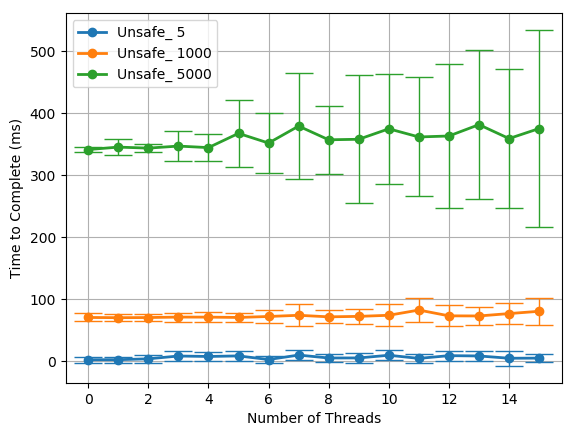
\includegraphics[scale=0.65]{step3_1.png}
\caption{Speed of the unsafe shared array when instantiated with various sizes}
\end{figure}


\begin{figure}\label{fig:step3_2}
\centering
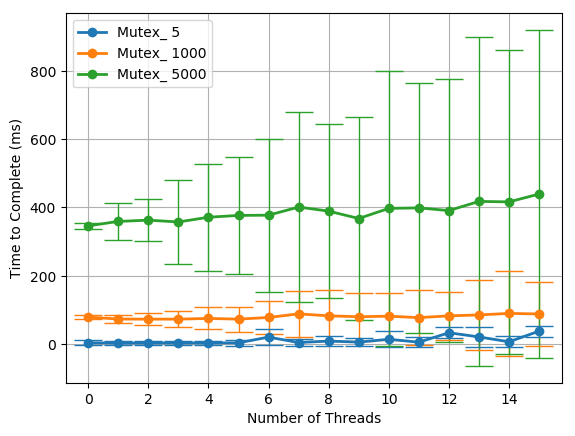
\includegraphics[scale=0.65]{step3_2.png}
\caption{Speed of the safe, mutex locked, shared array when instantiated with various sizes}
\end{figure}

The locked array (Fig \ref{fig:step3_2}) did not perform significantly worse in the average case than the unsafe array (Fig \ref{fig:step3_1}),
however the variance increases significantly as the number of threads and size of the array increases. I expect this is due to a one sided distribution, where the majority of results are scattered close to the mean with some large outliers which took much longer due to a delay in loading into local cache and taking a lock. The difference in standard deviation and means for the largest array size is shown in Fig \ref{fig:step3_3}. The fact that the mean time to complete does not increase substantially with increasing thread count suggests that the bottleneck for each loop in the common case is not taking the lock or running the sum operation but instead due to overheads like loading the array to cache to be summed and checking exit conditions for the loop.


\begin{figure}\label{fig:step3_3}
\centering
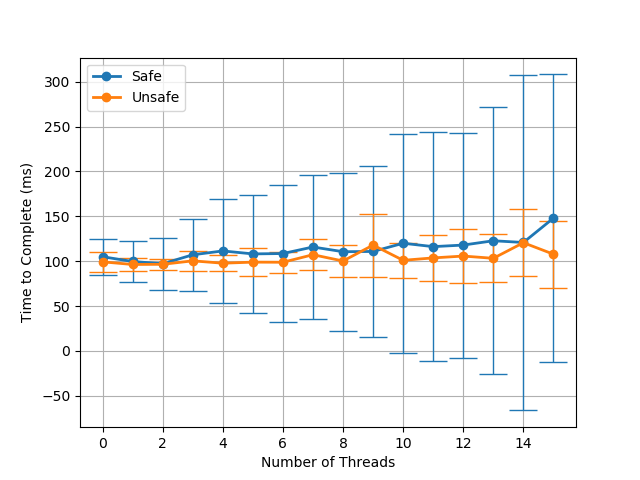
\includegraphics[scale=0.65]{step3_3.png}
\caption{Comparative speed of the unsafe and mutex-locked arrays set to a size of $X=5000$. The standard deviation is much more constant for the unsafe version.}
\end{figure}


\subsection{TATAS Lock}

\begin{figure}\label{fig:step4_1}
\centering
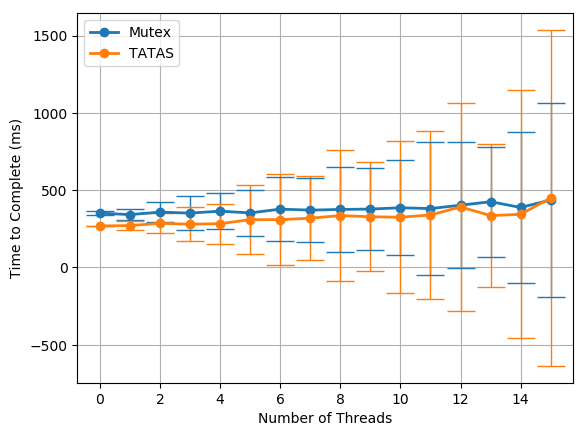
\includegraphics[scale=0.65]{step4_1.png}
\caption{Speed of the mutex-locked and TaTaS shared arrays for $X=5000$}
\end{figure}


The TaTaS-lock performed slightly better than the mutex-lock for small numbers of threads due to its better cache line behaviour, but as the number increased, the performance of the TaTaS lock deteriorated and the standard deviation of its operation increased greatly (Fig \ref{fig:step4_1}}).  This is potentially due to the overhead of having to do an extra test before test and setting, slightly delaying the operation of the code.

\todo{better explanation}

\subsection{Reader-Writer Lock}
\begin{figure}\label{fig:step5_1}
\centering
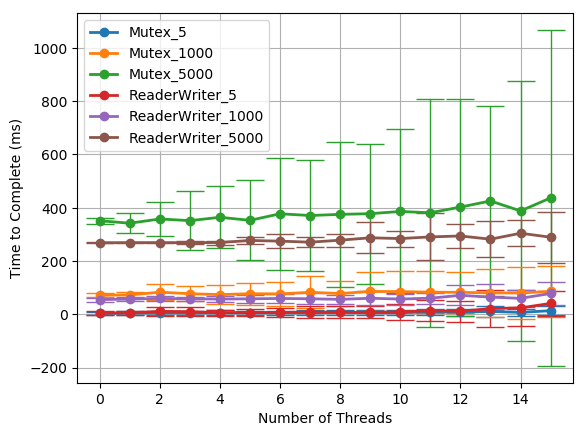
\includegraphics[scale=0.65]{step5_1.png}
\caption{Speed of the mutex-locked array versus the reader-writer locked array when instantiated with various sizes}
\end{figure}

\begin{figure}\label{fig:step5_2}
\centering
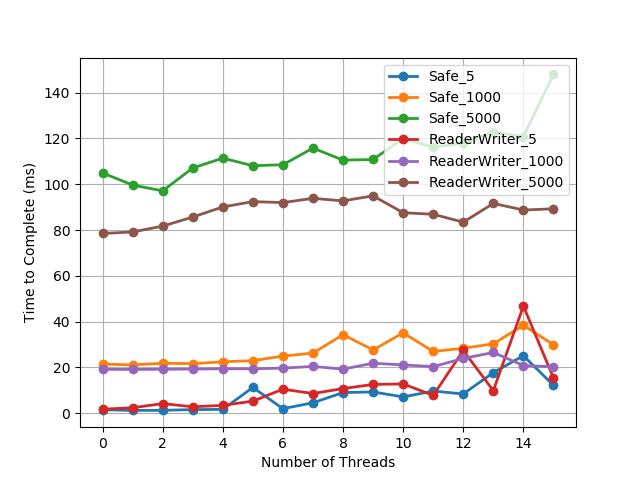
\includegraphics[scale=0.65]{step5_2.png}
\caption{Speed of the mutex-locked array versus the reader-writer locked array when instantiated with various sizes, drawn without error bars to more clearly show the mean-behaviour.}
\end{figure}

When the array size is not negligibly small, the reader-writer lock significantly outperforms the standard mutex lock as it allows multiple summing operations to occur at once. It also has a much smaller standard deviation for each operation than seen in mutex case (Figs \ref{fig:step5_1}, \ref{fig:step5_2}). This may be due to the much shorter array access delay time due to not having to wait for a lock on the array.

\subsection{Flag-Based Lock}

\begin{figure}\label{fig:step6_1}
\centering
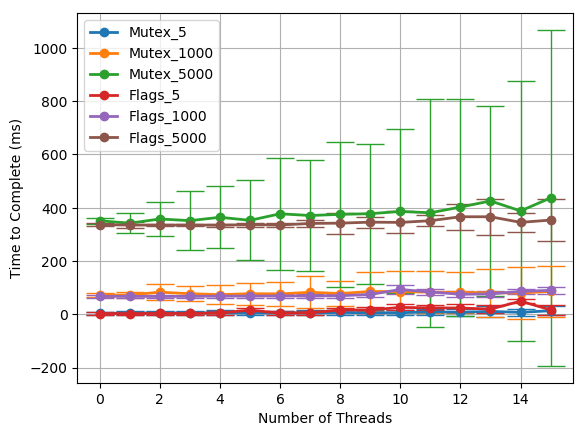
\includegraphics[scale=0.65]{step6_1.png}
\caption{Speed of the mutex-locked array versus the flag-locked array when instantiated with various sizes}
\end{figure}

The flag based lock outperformed the mutex-lock less significantly than the reader-writer lock but with a tighter standard deviation. \todo{clearer}

\begin{figure}\label{fig:step6_2}
\centering
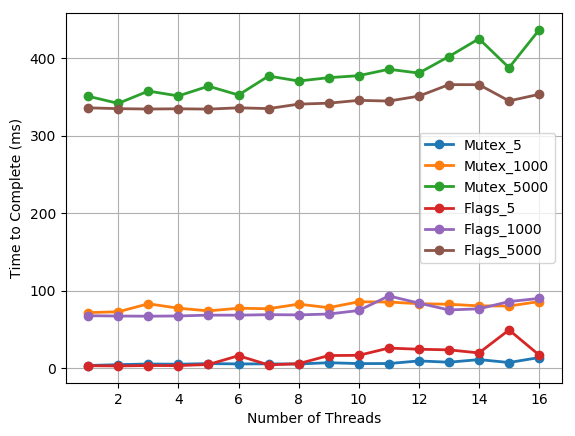
\includegraphics[scale=0.65]{step6_2.png}
\caption{Speed of the mutex-locked array versus the flag-locked array when instantiated with various sizes, drawn without error bars to more clearly show the mean-behaviour.}
\end{figure}

\subsection{Write Mode}

\begin{figure}\label{fig:step7_1}
\centering
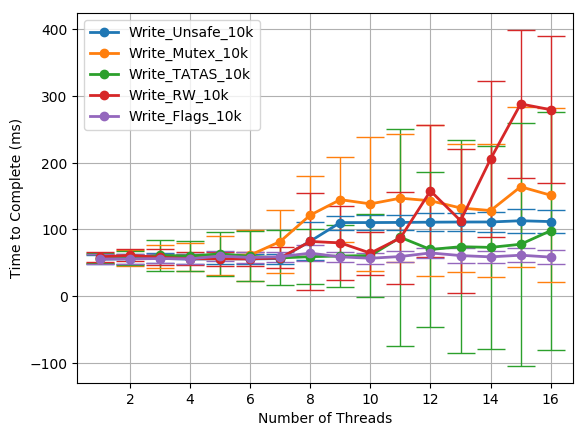
\includegraphics[scale=0.65]{step7_1.png}
\caption{Speed of the mutex-locked array versus the flag-locked array when instantiated with various sizes, drawn without error bars to more clearly show the mean-behaviour.}
\end{figure}

\begin{figure}\label{fig:step7_2}
\centering
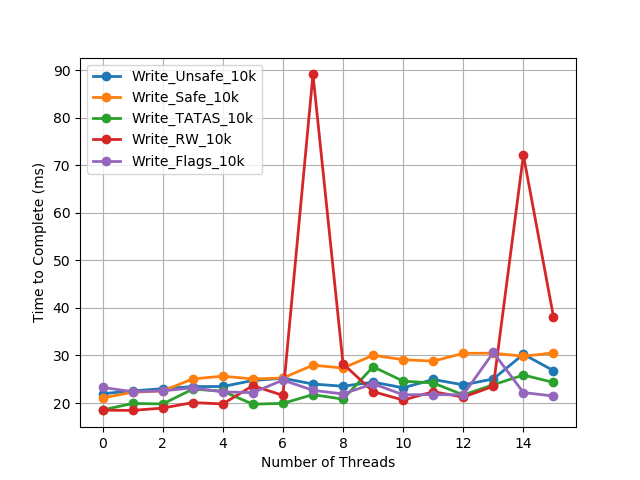
\includegraphics[scale=0.65]{step7_2.png}
\caption{Speed of the mutex-locked array versus the flag-locked array when instantiated with various sizes, drawn without error bars to more clearly show the mean-behaviour.}
\end{figure}

\begin{figure}\label{fig:step7_3}
\centering
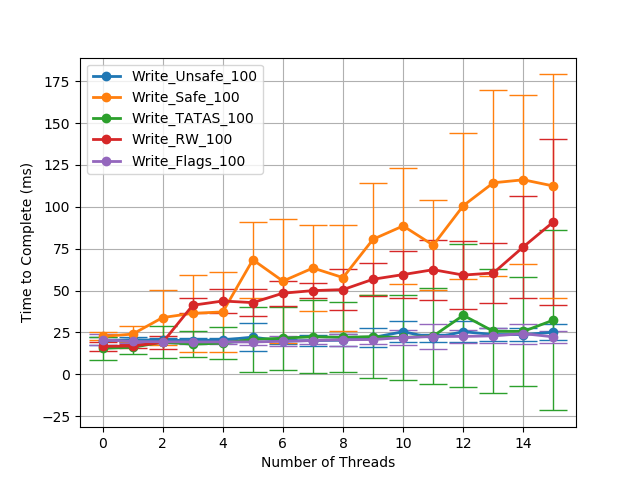
\includegraphics[scale=0.65]{step7_3.png}
\caption{Speed of the mutex-locked array versus the flag-locked array when instantiated with various sizes, drawn without error bars to more clearly show the mean-behaviour.}
\end{figure}

\begin{figure}\label{fig:step7_4}
\centering
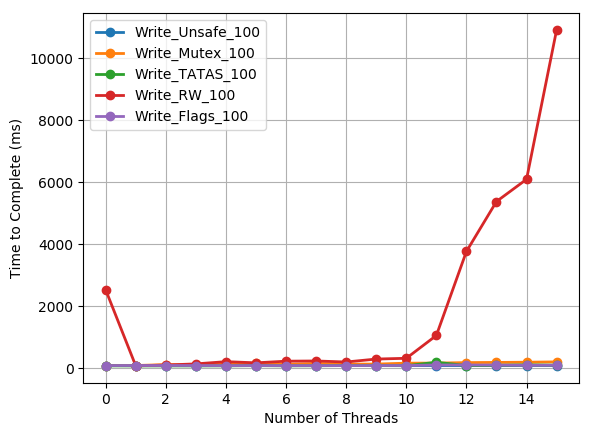
\includegraphics[scale=0.65]{step7_4.png}
\caption{Speed of the mutex-locked array versus the flag-locked array when instantiated with various sizes, drawn without error bars to more clearly show the mean-behaviour.}
\end{figure}




\section{Summary}

\end{document}